%% Assignment
%% 中文报告、作业报告、实验报告、文献
%%%%%%%%%%%%%%%%%%%%%%%%%%%%%%%%%%%%%%%%%

%----------------------------------------------------------------------------------------
%	PACKAGES AND OTHER DOCUMENT CONFIGURATIONS
%----------------------------------------------------------------------------------------

\documentclass[UTF8]{ctexart}
%%%%%%%%%%%%%%%%%%%%%%%%%%%%%%%%%%%%%%%%%
% Lachaise Assignment
% Structure Specification File
% Version 1.0 (26/6/2018)
%
% This template originates from:
% http://www.LaTeXTemplates.com
%
% Authors:
% Marion Lachaise & François Févotte
% Vel (vel@LaTeXTemplates.com)
%
% License:
% CC BY-NC-SA 3.0 (http://creativecommons.org/licenses/by-nc-sa/3.0/)
% 
%%%%%%%%%%%%%%%%%%%%%%%%%%%%%%%%%%%%%%%%%

%----------------------------------------------------------------------------------------
%	PACKAGES AND OTHER DOCUMENT CONFIGURATIONS
%----------------------------------------------------------------------------------------

\usepackage{amsmath,amsfonts,stmaryrd,amssymb} % Math packages

\usepackage{enumerate} % Custom item numbers for enumerations

\usepackage[ruled]{algorithm2e} % Algorithms

\usepackage[framemethod=tikz]{mdframed} % Allows defining custom boxed/framed environments

\usepackage{listings} % File listings, with syntax highlighting
\lstset{
	basicstyle=\ttfamily, % Typeset listings in monospace font
}
\usepackage{indentfirst}
\usepackage{bm}  %给数学符号加粗
\usepackage[colorlinks,  %引入超链接
linkcolor=black,
anchorcolor=black,
citecolor=black,
urlcolor=black
]{hyperref}
%----------------------------------------------------------------------------------------
%	DOCUMENT MARGINS
%----------------------------------------------------------------------------------------
%使图片、表格的编号按照section重新开始
%\usepackage{amsmath}
%\numberwithin{figure}{section}
%\numberwithin{table}{section}
%使section的标题左对齐
\CTEXsetup[format={\Large\bfseries}]{section}
\usepackage{geometry} % Required for adjusting page dimensions and margins

\geometry{
	paper=a4paper, % Paper size, change to letterpaper for US letter size
	top=2.5cm, % Top margin
	bottom=3cm, % Bottom margin
	left=2.5cm, % Left margin
	right=2.5cm, % Right margin
	headheight=14pt, % Header height
	footskip=1.5cm, % Space from the bottom margin to the baseline of the footer
	headsep=1.2cm, % Space from the top margin to the baseline of the header
	%showframe, % Uncomment to show how the type block is set on the page
}

\usepackage{fancyhdr}  %%设置页眉页脚
\pagestyle{fancy}   %风格为fancy(便于自己定义)
\fancyhead[L]{}  %左页眉为空
\fancyfoot{}   %页脚为空
\fancyfoot[C]{\thepage}  %页脚中间为页数
\renewcommand{\headrulewidth}{0pt} %去掉页眉下的横线

% 表格中支持跨行
\usepackage{multirow}

% 跨页表格
\usepackage{longtable}

% 固定宽度的表格
\usepackage{tabularx}

\usepackage{booktabs}

% 表格中的反斜线
\usepackage{diagbox}

% 确定浮动对象的位置,可以使用 H,强制将浮动对象放到这里(可能效果很差)
\usepackage{float}

%\usepackage{natbib}

\graphicspath{{figures/}}

%----------------------------------------------------------------------------------------
%	FONTS
%----------------------------------------------------------------------------------------
\usepackage{setspace}

\usepackage[utf8]{inputenc} % Required for inputting international characters
\usepackage[T1]{fontenc} % Output font encoding for international characters

\usepackage{XCharter} % Use the XCharter fonts
\usepackage{color}   %改变字体颜色
\usepackage{url}   %引用网址
\usepackage{bm}  %给数学符号加粗
\usepackage{subfigure} %have figures within figures
\usepackage{graphicx}
%\usepackage{wrapfig}  %插入图片
%----------------------------------------------------------------------------------------
%	COMMAND LINE ENVIRONMENT
%----------------------------------------------------------------------------------------

% Usage:
% \begin{commandline}
%	\begin{verbatim}
%		$ ls
%		
%		Applications	Desktop	...
%	\end{verbatim}
% \end{commandline}

\mdfdefinestyle{commandline}{
	leftmargin=10pt,
	rightmargin=10pt,
	innerleftmargin=15pt,
	middlelinecolor=black!50!white,
	middlelinewidth=2pt,
	frametitlerule=false,
	backgroundcolor=black!5!white,
	frametitle={Command Line},
	frametitlefont={\normalfont\sffamily\color{white}\hspace{-1em}},
	frametitlebackgroundcolor=black!50!white,
	nobreak,
}

% Define a custom environment for command-line snapshots
\newenvironment{commandline}{
	\medskip
	\begin{mdframed}[style=commandline]
}{
	\end{mdframed}
	\medskip
}

%----------------------------------------------------------------------------------------
%	FILE CONTENTS ENVIRONMENT
%----------------------------------------------------------------------------------------

% Usage:
% \begin{file}[optional filename, defaults to "File"]
%	File contents, for example, with a listings environment
% \end{file}

\mdfdefinestyle{file}{
	innertopmargin=1.6\baselineskip,
	innerbottommargin=0.8\baselineskip,
	topline=false, bottomline=false,
	leftline=false, rightline=false,
	leftmargin=2cm,
	rightmargin=2cm,
	singleextra={%
		\draw[fill=black!10!white](P)++(0,-1.2em)rectangle(P-|O);
		\node[anchor=north west]
		at(P-|O){\ttfamily\mdfilename};
		%
		\def\l{3em}
		\draw(O-|P)++(-\l,0)--++(\l,\l)--(P)--(P-|O)--(O)--cycle;
		\draw(O-|P)++(-\l,0)--++(0,\l)--++(\l,0);
	},
	nobreak,
}

% Define a custom environment for file contents
\newenvironment{file}[1][File]{ % Set the default filename to "File"
	\medskip
	\newcommand{\mdfilename}{#1}
	\begin{mdframed}[style=file]
}{
	\end{mdframed}
	\medskip
}

%----------------------------------------------------------------------------------------
%	NUMBERED QUESTIONS ENVIRONMENT
%----------------------------------------------------------------------------------------

% Usage:
% \begin{question}[optional title]
%	Question contents
% \end{question}

\mdfdefinestyle{question}{
	innertopmargin=1.2\baselineskip,
	innerbottommargin=0.8\baselineskip,
	roundcorner=5pt,
	nobreak,
	singleextra={%
		\draw(P-|O)node[xshift=1em,anchor=west,fill=white,draw,rounded corners=5pt]{%
		Question \theQuestion\questionTitle};
	},
}

\newcounter{Question} % Stores the current question number that gets iterated with each new question

% Define a custom environment for numbered questions
\newenvironment{question}[1][\unskip]{
	\bigskip
	\stepcounter{Question}
	\newcommand{\questionTitle}{~#1}
	\begin{mdframed}[style=question]
}{
	\end{mdframed}
	\medskip
}

%----------------------------------------------------------------------------------------
%	WARNING TEXT ENVIRONMENT
%----------------------------------------------------------------------------------------

% Usage:
% \begin{warn}[optional title, defaults to "Warning:"]
%	Contents
% \end{warn}

\mdfdefinestyle{warning}{
	topline=false, bottomline=false,
	leftline=false, rightline=false,
	nobreak,
	singleextra={%
		\draw(P-|O)++(-0.5em,0)node(tmp1){};
		\draw(P-|O)++(0.5em,0)node(tmp2){};
		\fill[black,rotate around={45:(P-|O)}](tmp1)rectangle(tmp2);
		\node at(P-|O){\color{white}\scriptsize\bf !};
		\draw[very thick](P-|O)++(0,-1em)--(O);%--(O-|P);
	}
}

% Define a custom environment for warning text
\newenvironment{warn}[1][Warning:]{ % Set the default warning to "Warning:"
	\medskip
	\begin{mdframed}[style=warning]
		\noindent{\textbf{#1}}
}{
	\end{mdframed}
}

%----------------------------------------------------------------------------------------
%	INFORMATION ENVIRONMENT
%----------------------------------------------------------------------------------------

% Usage:
% \begin{info}[optional title, defaults to "Info:"]
% 	contents
% 	\end{info}

\mdfdefinestyle{info}{%
	topline=false, bottomline=false,
	leftline=false, rightline=false,
	nobreak,
	singleextra={%
		\fill[black](P-|O)circle[radius=0.4em];
		\node at(P-|O){\color{white}\scriptsize\bf i};
		\draw[very thick](P-|O)++(0,-0.8em)--(O);%--(O-|P);
	}
}

% Define a custom environment for information
\newenvironment{info}[1][Info:]{ % Set the default title to "Info:"
	\medskip
	\begin{mdframed}[style=info]
		\noindent{\textbf{#1}}
}{
	\end{mdframed}
}
 % Include the file specifying the document structure and custom commands

%----------------------------------------------------------------------------------------
%	ASSIGNMENT INFORMATION
%----------------------------------------------------------------------------------------

\title{降雨量预测} % Title of the assignment

\author{孟诗涵$\;\;$ 2019211246\\张芙作$\;\;$2019211220} % Author name and email address

\date{} % University, school and/or department name(s) and a date

%----------------------------------------------------------------------------------------

\begin{document}\normalsize

\maketitle % Print the title
\setlength{\baselineskip}{18pt}
%----------------------------------------------------------------------------------------
\begin{abstract}
  降雨量预测在农业、交通、社会管理等领域都有非常实际的应用价值,一直备受学界和工业界所关注。
  在本次项目中,我们以数据驱动的方法为基础,根据历史的气象数据对未来的降雨量进行预测。
  具体的,根据当地气象站前六时刻的气象数据对未来下一时刻的降雨量类别进行预测,可能的降雨情况
  有:无雨,小雨,中雨,大雨到暴雨共4种。为了对未来降雨量给出精确的预测,尝试了不同的分类模型,
  主要采用了线性模型、树模型和神经网络三大类机器学习方法。为了进一步提高模型的预测能力,将
  单独的分类模型用不同的集成学习方法组合成更大的分类器。在所选的五个气象站上分别用以上所有方法
  训练分类器,并通过验证集对模型进行选择,并用四种不同的指标对分类器进行评价。
  实验结果显示不同模型在该问题上的预测精度无显著差别,比较之下GBDT模型的预测能力稍高一些,而
  用voting和bagging的方式对模型进行组合对单独模型的预测能力没有明显提高。
  \\

\textbf{关键字:}降雨量预测;分类;机器学习;集成学习
\end{abstract}

\section{简介}
降雨量任务属于时空序列类预测问题,由于该问题的研究具有实际的应用价值和意义,所以一直以来
备受学界和工业界的关注。气象参数之间往往存在这非常复杂的相互关系,而且降雨量本身存在
不确定性和随机性,因此降雨量预测是一个非常有难度的任务。
降雨量预测中,根据研究思路的区分主要有数值天气预报模型和遥感观测两种方法\cite{bit1},后者主要是基于
专业领域的气象观测而获得的,在这里不作讨论。

基于天气数据对降雨量进行预测的方法早期有基于统计模型的线性模型、多元线性回归等,之后随着
机器学习算法的发展和广泛应用,有研究者用人工神经网络进行短期的降雨量预测。由于用单个模型
进行预测结果往往不尽人意,有学者采用混合模型的方法来实现降雨量预测,比如将K近邻,人工神经
网络模型的结果通过加权平均来进行预测,从而避免单个模型的不稳定性。文献\cite{bit3}分别用
线性回归模型和神经网络来对局部以及全局气象数据进行建模,并分别进行预测,并通过动态的组合方法
将两种预测器预测的结果进行组合,基于这样的组合模型对空气质量中的PM2.5进行预测,
并给予这样的模型实现了在线的预测工具。文献\cite{bit4}结合了小波变换技术和神经网络模型来解决
降雨量预测问题。
不仅仅是传统的机器学习算法,近年来由于深度学习在时间序列问题上有了非常成功的应用
开始有研究者将深度学习模型引入到时间序列的降雨量预测问题上,以实现端到端的
建模和预测。
文献\cite{bit5}中提出了一种用于时空序列数据处理的深度网络预测模型,引入了多层卷积神经网络
来提取时间上的变化趋势和空间上的距离相关性,并将时空特征融合进一步预测。
文献\cite{bit2}中采用了双层LSTM网络结构来实现基于时空序列数据的空气质量预测和降雨量预测,
为了提高模型的拟合能力,同时引入了注意力机制对不同的特征赋予不同的权重,从而自动提取其他检测变量与
目标变量之间的动态相关性。与其他的基于统计模型或者智能算法的方法相比,采用如LSTM这种循环神经网络的
方法可以方便的对时间序列进行处理,无需过多的数据预处理,可以完整保留数据在时间上的变化特性和变量在时间
上的相关性。所以越来越多的学者开始尝试用循环神经网络来处理时空序列问题。

在本次项目中,我们将降雨量预测问题定义为通过前六时刻的气象数据对当地下一时刻的降雨量类别进行预测的
分类问题,我们分别采用了线性分类器、基于决策树的分类算法以及基于神经网络的模型来解决降雨量预测问题,并通过对不同模型的组合
来进一步得到拟合能力更高的模型。我们对五个在同一个城市的不同气象站分别用模型对当地的气象特点进行建模,
分别对当地的降雨量进行预测,并对采用了不同模型的分类器结果进行了比较和分析。

\section{任务定义}
本文将降水量预测问题定义为分类问题,按照表\ref{tab:jyl}中所示的标准根据降水量的数值分成无雨,小雨,中雨和大
到暴雨四类: 

\begin{table}[htb]
  \centering
  \begin{minipage}[t]{\linewidth}
  \centering
  \caption{降雨量分类标准}
  \label{tab:jyl}
    \begin{tabular}{ccccc}
      \toprule[1pt]
      降雨量(毫米/小时) & 0 & (0,1] & (1,4] & (4,$\infty$) \\
      \midrule[0.5pt]
      类别 & 无雨 & 小雨 & 中雨 & 大到暴雨\\
      标号 & 0 & 1 & 2 & 3\\
      \bottomrule[1pt]
    \end{tabular}
  \end{minipage}
\end{table}

同时,本文将问题定义为短时预测问题,基于前六小时的特征数据预测下一小时的降
水量,对 5 个邻近气象站分别单独建模。

获得的原始数据为每个气象站按照时间顺序每个时刻(一小时一个采用)的气象特征监测值,
从第一个有记录的时刻开始进行窗口滑动,窗口滑动的步伐为1,当前时刻到
之后的连续第6个时刻的数据样本作为一个样本,第7时刻的降雨量类别作为该样本的目标值。
这样将每一个样本都是一个二维的$T\times P$矩阵,其中$T$为时间周期,在这里为6,$P$
为每一个时刻所选用的特征个数。所以当共有$N$个样本时,降雨量预测任务的输入为$N$个
样本的特征,即为$N\times T\times P$的数据集,希望降雨量预测模型能够根据每一个样本
给出该样本所示的前六个时刻的气象数据给出下一时刻的降雨量类别预测,这样模型
对所有$N$个输入样本的输出为一个长度为$N$的类别向量。

\section{数据整理}
\subsection{数据来源及内容}
\label{sec:data}
数据集来自巴西国家气象研究所(INMET),它涵盖了来自东南地区(巴西)的122个气象站从2000年到2016年的每小时天气观测数据(并非所有气象站都是从2000年开始观测的)。东南部包括里约热内卢,圣保罗,米纳斯吉拉斯州和圣埃斯皮里图州等。数据是由维萨拉自动气象站AWS310自动捕捉,所以可能发生设备故障导致数据错误或缺失的情况。整个数据集规模为9779168条信息,31个特征。 其中有时间地点,气象站编号等信息,还有17个气象数据分别为temp-瞬时空气温度(摄氏度)、tmax-最高气温(摄氏度)、tmin-最低气温(摄氏度)、hmdy-空气相对湿度(%)。hmax-最大相对空气湿度(%)、hmin-最低相对空气湿度(%)、dewp-即时露点(摄氏度)、dmax-最大露点(摄氏度)、dmin-最低露点温度(摄氏度)、stp-瞬时大气压(百帕)、smax-最大大气压(百帕)、smin-最低大气压(百帕)、wdsp-瞬时风速(米/秒)、wdct-风向(半径度)、gust-阵风强度(米/秒)、gbrd-太阳辐射、prcp-降水量(毫米)。

首先观察气象数据的分布,最大值最小值应与实际值有类似的分布,具体见图\ref{fig:1}。其中所有特征均有较多的零值,需要逐一分析,并进行对应的清洗。需要预测的prcp-降水量绝大部分都是0值,非常稀疏,给预测带来了很大的困难。stp-气压、temp-温度、dewp-露点温度基本为正态分布,数值保持在一个范围之内。考虑到夜晚没有太阳照射,gbrd-太阳辐射绝大部分值为0,低辐射值分布略比高辐射值大,中辐射值分布比较均匀。hmdy-空气湿度数值从100\%降低,分布越来越少。风速是一个均值偏向0的正态分布。

\begin{figure}[htbp]
\label{fig:1}
\centering

\subfigure[prcp-降水量]{
\begin{minipage}[t]{0.33\linewidth}
\centering
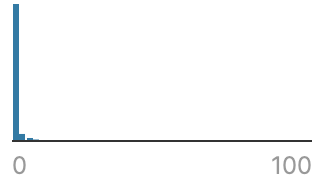
\includegraphics[width=0.8\textwidth]{1-1.png}
%\caption{fig1}
\end{minipage}%
}%
\subfigure[stp-气压]{
\begin{minipage}[t]{0.33\linewidth}
\centering
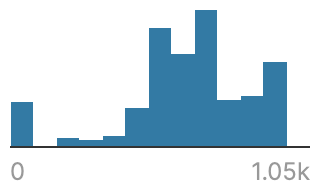
\includegraphics[width=0.8\textwidth]{1-2.png}
%\caption{fig2}
\end{minipage}%
}%        
\subfigure[gbrd-太阳辐射]{
\begin{minipage}[t]{0.33\linewidth}
\centering
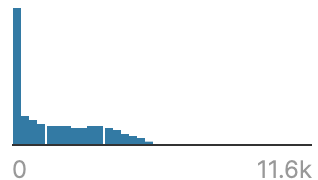
\includegraphics[width=0.8\textwidth]{1-3.png}
%\caption{fig2}
\end{minipage}
}%
\quad  
\subfigure[temp-空气温度]{
\begin{minipage}[t]{0.33\linewidth}
\centering
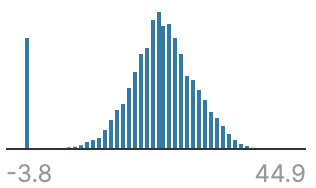
\includegraphics[width=0.8\textwidth]{1-4.png}
%\caption{fig2}
\end{minipage}
}%
\subfigure[dewp-露点温度]{
\begin{minipage}[t]{0.33\linewidth}
\centering
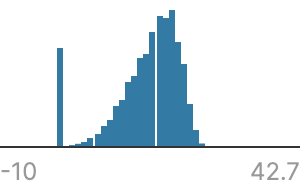
\includegraphics[width=0.8\textwidth]{1-5.png}
%\caption{fig2}
\end{minipage}
}%
\subfigure[hmdy-空气相对湿度]{
\begin{minipage}[t]{0.33\linewidth}
\centering
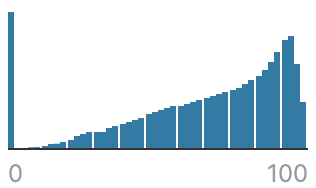
\includegraphics[width=0.8\textwidth]{1-6.png}
%\caption{fig2}
\end{minipage}
}%
\quad
\subfigure[wdsp-瞬时风速]{
\begin{minipage}[t]{0.33\linewidth}
\centering
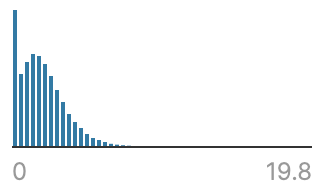
\includegraphics[width=0.8\textwidth]{1-7.png}
%\caption{fig2}
\end{minipage}
}%
\subfigure[wdct-风向]{
\begin{minipage}[t]{0.33\linewidth}
\centering
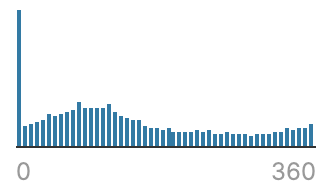
\includegraphics[width=0.8\textwidth]{1-8.png}
%\caption{fig2}
\end{minipage}
}%
\subfigure[gust-阵风]{
\begin{minipage}[t]{0.33\linewidth}
\centering
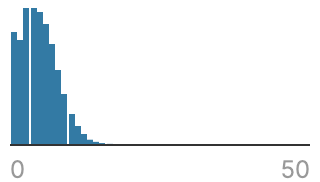
\includegraphics[width=0.8\textwidth]{1-9.png}
%\caption{fig2}
\end{minipage}
}%

\centering
\caption{各气象特征数据分布直方图\cite{bit6}}
\end{figure}

\subsection{数据清洗及处理}

对不同的参数有不同的处理。其中降水量和太阳能将nan值用0替代,作为可用数据条。Stp,smax,smin表示气压值,temp,tmax,tmin, dewp, dmax, dmin表示温度,hmdy, hmax, hmin表示湿度,wdsp,wdct,gust表示风速有关的数据。上述特征值均为连续实数,将nan值用0替代后做线性插值,但是线性插值对长时间一整段的数据缺失无用,所以进一步的清洗可以直接将一整段数据丢失的样本丢弃。

有一个气象站的经纬度及海拔信息缺失,谷歌出正确的信息补全。另外有两个气象站经纬度信息错误,改正。

考虑到计算机算力问题,在122个气象站中根据数据量排序选择编号为371-375的五个气象站,它们均在RJ省,经纬度上看为邻近的城市,海拔均在100米以下,靠近海边,受热带气候影响,降雨量较多,一定程度上缓解数据稀疏问题,有利于模型分类。

\section{特征处理}
\subsection{数据归一化处理}
采用sklearn包中standardScaler对数据统一进行归一化处理,变为标准正态分布。即默认训练集验证集测试集同分布。本文采用的某些模型对归一化不敏感,有些则很敏感,这是由模型结构本身决定的,具体说明见章节\ref{sec:model design}。

\subsection{最终使用的特征维度和每一维的含义}
\label{feature_subset}
气象数据中大气压、温度、湿度在一个小时内基本稳定,所以将最大值最小值丢弃,只采用stp、temp、dewp、hmdy、wdsp、wdct、gust等进行建模。保留时间特征,因为时间序列中时间是非常重要的特征,反应了待预测数据量的变化信息。另外考虑到五个气象站的不同,保留地理位置等信息,最终单个气象站模型使用的特征共13维,具体见表\ref{tab:feature}。在章节\ref{sec:all features}会讨论全部特征和进行选择后的部分特征对结果造成的影响。

\begin{table}[htb]
  \centering
  \begin{minipage}[t]{0.4\linewidth}
  \caption{最终使用的特征}{}
  \label{tab:feature}
    \begin{tabular}{cc}
      \toprule[1.5pt]
      特征名称& {特征含义} \\
      \midrule[1pt]
      {yr} & 年 \\
      {mo} & 月  \\
      {da} & 日 \\
      {hr} & 小时  \\
      {stp} & 气压 \\
      {gbrd} & 太阳辐射 \\
      {temp} & 空气温度 \\
      {dewp} & 露点温度 \\
      {hmdy} & 空气相对湿度 \\
      {wdsp} & 瞬时风速 \\
      {wdct} & 风向 \\
      {gust} & 阵风强度 \\
      {prcp} & 过去一小时降水量 \\
      \bottomrule[1.5pt]
    \end{tabular}
  \end{minipage}
\end{table}

\subsection{特征相关性}
在整个数据集上观察各个特征维度与预测值降水量的相关性,得到结果如图\ref{fig:corr}所示。由图可得到以下结论:
\begin{itemize}
	\item 最大值最小值相关性基本与实际值相等,说明之前的特征选择操作是合理的;
	\item 湿度hmdy,阵风gust等与降水量prcp正相关;太阳辐射gbrd,温度temp,气压stp与降水量prcp负相关,即风大气压低更有可能下雨,基本符合常识;
	\item 时间,经纬度和气象站信息相关性相对不明显。
\end{itemize}


\begin{figure}[h] % use float package if you want it here
  \centering
  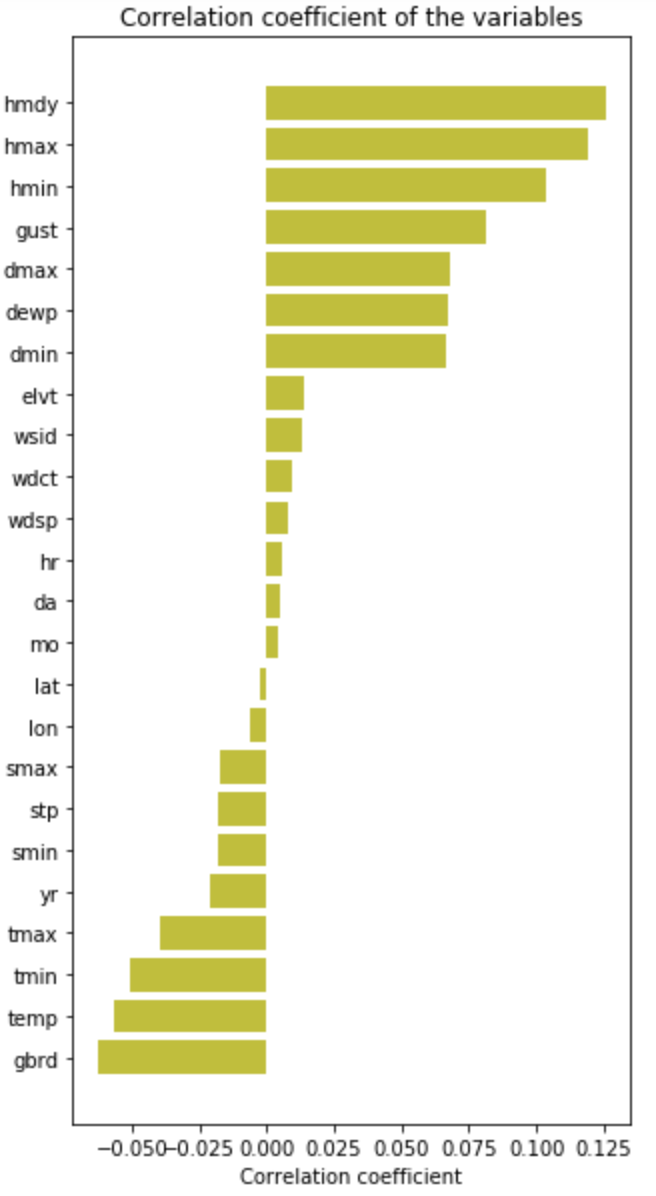
\includegraphics[width = 0.4\textwidth]{corr.png}
  \caption{特征相关性}
  \label{fig:corr}
\end{figure}

因为降水量为时间序列,为了观察时序上的相关性,以温度temp和湿度hmdy为例,得到相关性热度图如图\ref{fig:timelag}所示。可以得到如下结论:
\begin{itemize}
	\item 湿度hmdy和温度temp均有明显的时间正相关性,时间越近相关性越大,接近1;
	\item 湿度hmdy和温度temp有明显的负相关性。
\end{itemize}

\begin{figure}[h] % use float package if you want it here
  \centering
  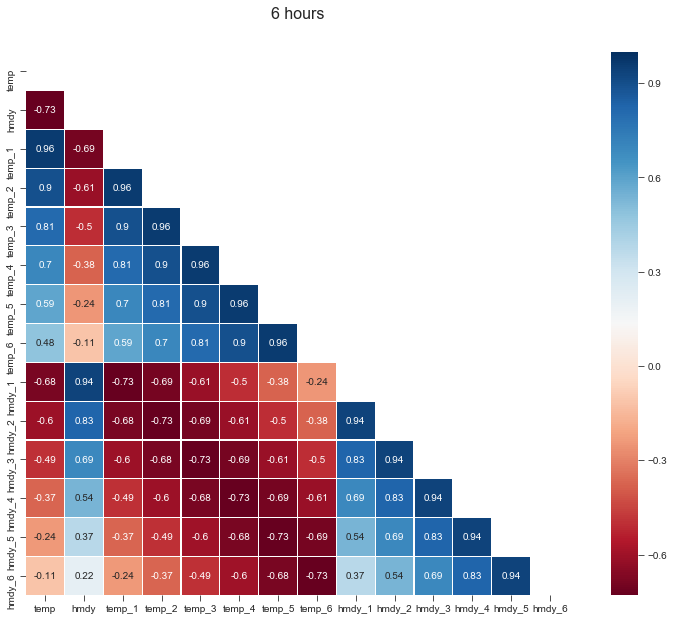
\includegraphics[width = 0.8\textwidth]{time-lag.png}
  \caption{6小时内温度和湿度相关性热度图}
  \label{fig:timelag}
\end{figure}

\section{模型设计}
\label{sec:model design}
\subsection{线性模型}

\subsubsection{逻辑回归分类器Logistic Regression Classifier}

逻辑回归假设数据服从伯努利分布,通过极大化似然函数方法,运用梯度下降来求解参数,来达到将数据二分目的。多分类器可由二分类器推广得到。本质上是一个线性模型,可利用特征核函数将低维特征映射到高维,类似支持向量机(SVM)。


逻辑回归分类器具有如下优点:
\begin{enumerate}[(1)]
	\item 直接对分类的可能性建模,无需事先假设数据分布,避免了假设分布不准确带来的问题。同时对率函数是任意阶可导凸函数,有很好得数学性质,很多数值优化算法可直接用于求取最优解;
	\item 不仅预测出类别,还可得到近似概率预测,因此可用作排序模型;
	\item 算法简单,容易使用和解释,计算代价低,可应用于分布式数据和在线算法实现,用较小资源处理较大数据;
	\item 算法稳定性高,对数据中小噪声鲁棒性很好,并且不会受到轻微多重共线性影响。
\end{enumerate}

缺点:
\begin{enumerate}[(1)]
	\item 容易欠拟合,分类精度不高;
	\item 数据特征有缺失或特征空间很大时效果不好。
\end{enumerate}


\subsubsection{SVM}
支持向量机(support vector machine,SVM)是一种二分类模型,可推广到多分类器。其基本模型定义是特征空间上的间隔最大的线性分类器(当采用线性核时),即支持向量机的学习策略是间隔最大化,最终可转化为一个凸二次规划问题的求解。对于线性不可分问题,可利用核函数将低维特征映射到高维,再进行划分。

支持向量机算法具有如下优点:
\begin{enumerate}[(1)]
	\item SVM算法简单,易于理解,核心为最大化分类边界,得到支持向量;
	\item SVM 的最终决策函数只由少数的支持向量所确定,计算的复杂性取决于支持向量的数目,而不是样本空间的维数,这在某种意义上避免了“维数灾难”;
	\item 少数支持向量使算法具有较好的稳定性,比如增删非支持向量样本对模型没有影响。
\end{enumerate}

缺点:
\begin{enumerate}[(1)]
	\item 通过二次规划来求解计算复杂度高,大样本时所需时间长;
	\item 非线性问题的核函数难以选择;
	\item 对缺失数据敏感。
\end{enumerate}


\subsubsection{KNN}
KNN是近邻法的一种,核心思想为一个样本的分类结果与它周围的邻居类别有关,通过投票法等方法确定该样本的类别。

近邻法具有如下优点:
\begin{enumerate}[(1)]
	\item 算法简单,易于理解,易于实现,无需估计参数,无需训练;
	\item 适合于多分类问题(multi-modal,对象具有多个类别标签)。
\end{enumerate}

缺点:
\begin{enumerate}[(1)]
	\item 需要存储所有样本的距离矩阵,计算量大,内存开销大;
	\item 样本不平衡时,对稀有类别的预测准确率低;
	\item 相比于决策树模型,可解释性不强。
\end{enumerate}


\subsection{树模型}

\subsubsection{Decision Tree}
决策树是基于规则进行决策和判别的树模型,目的是构造一棵泛化能力强的树。它采用自顶向下的递归方式来生长。随着树的生长,完成对训练样本集的不断细分,最终都被细分到了每个叶子结点上。


决策树具有如下优点:
\begin{enumerate}[(1)]
	\item 对噪声数据具有很好的鲁棒性,且对缺失值不敏感,能处理连续离散等多种属性的数据;
	\item 效率高,运行时间短,一旦构建完决策树模型,可以多次使用;
	\item 学习得到的决策树可以表示为多条if-then形式的决策规则,因此具有很强的可读性和可解释性。
\end{enumerate}

缺点:
\begin{enumerate}[(1)]
	\item 容易导致过拟合,需要剪枝等操作,或者采用随机森林模型;
	\item 容易忽略数据集中属性的相互关联,特别是在本文的时间序列模型中;
	\item 样本不均衡时,不同的判定准则会有不同的属性偏向:比如信息增益准则对数目较多的属性有所偏好(典型代表ID3算法),而增益率准则(CART)则对数目较少的属性有所偏好。
\end{enumerate}


\subsubsection{Random Forest}
随机森林是一个用随机方式建立的,包含多个决策树的分类器,也属于集成学习中的bagging算法的一种。随机性主要体现在两个方面:一是重采样,训练每棵树时,从全部训练样本(样本数为N)中选取一个可能有重复的大小同样为N的数据集进行训练(即bootstrap取样);二是随机选取特征,在每个节点,随机选取所有特征的一个子集,用来计算最优分类特征。

随机森林在决策树优缺点的基础上,具有不易过拟合,可以降低方差等优点,同时对于样本不均衡的问题,它可以平衡误差。


\subsubsection{GBDT}
GBDT是梯度下降与决策树模型的结合,是一种boosting方法,每一次建立模型,是在之前建立模型损失函数的梯度下降方向。

GBDT在决策树的基础上具有如下优点:
\begin{enumerate}[(1)]
	\item 具有boosting思想,每一步的残差计算其实变相地增大了分错实例(instance)的权重,而已经分对的实例(instance)则都趋向于0。这样后面的树就能越来越专注那些前面被分错的实例(instance);
	\item 表达能力强,无须对特征进行复杂的变换和选择,且能够自动对特征重要性排序。
\end{enumerate}

缺点:
\begin{enumerate}[(1)]
	\item Boost是一个串行过程,不好并行化,计算复杂度高;
	\item 不太适合高维稀疏特征,如果feature个数太多,每一棵回归树都要耗费大量时间,甚至不如SVM。
	
\end{enumerate}

\subsubsection{Xgboost}
XGBoost是Boosting算法的由多个弱决策分类树组成的一个强分类器。
类似于基本的CART树一样,通过不断地特征分裂来完成一棵决策树的构造,
为了对给定的损失函数进行最小化,采用贪心算法对每次节点分裂时的特征进行
选择。与传统的CART树采用不纯度等损失函数构造决策树不同,XGBoost中决策树
的构造可以根据需要设置目标函数,并且一般来讲,目标函数由两部分组成。
第一部分衡量预测类别和真实类别之间的差距,而另一部分则是正则化项,用于
控制模型的复杂度,防止模型出现过拟合,提高了最终分类器的泛化能力。
XGBoost基于Boosting思想采用串行方法产生多个决策树,每一次添加新的树,都是
去拟合上一次预测的残差,这样通过多次迭代产生一系列决策树组成一个大的分类器。

XGBoost算法是机器学习界的一大利器,被广泛应用于大数据竞赛和工程,其
作为一种特殊的集成树算法,拥有许多出色的优点:
\begin{enumerate}[(1)]
    \item 增加了很多防止过拟合的策略,比如目标函数中增加正则化项,对数据进行随机采样等;
    \item 在训练新的决策树时利用了损失函数的二阶导数,加快了优化速度
    \item 虽然基于Boosting思想树与树之间是串行关系,但是单个树的节点分裂过程可以实现并行
    化,用多线程来选择最佳分裂点,非常有效的加快了训练速度。
\end{enumerate}

当然,作为一种基于决策树的算法,与众多树算法相同,XGBoost的决策树训练也采用了贪心算法,相对
来说增加了训练过程的时间,另外由于XGBoost算法参数较多,在实际应用中需要较多的精力用来调参。

\subsection{神经网络模型}

\subsubsection{MLP}
MLP多层感知机是一种前馈神经网络,基于反向梯度传播学习。

MLP具有如下优点:
\begin{enumerate}[(1)]
	\item 高度的并行处理,算法效率高
	\item 有很强的自适应,自学习的能力。
\end{enumerate}

缺点:
\begin{enumerate}[(1)]
	\item 具有神经网络模型的统一缺点,可解释性较差;
	\item 网络隐含层的参数选取比较困难,容易陷入局部极值。
	
\end{enumerate}

\subsubsection{LSTM}

LSTM(长短时记忆网络)是一种特殊的循环神经网络,其被广泛用于时间序列问题,特别是
在自然语言处理问题上有非常突出的表现。
由于LSTM网络的输入具有明确的时间先后关系,所以适合处理本项目中具有明显时间轴信息
的时间序列数据。为了根据前六小时的天气状况预测当地下一时刻的降雨量,用多层的LSTM网络
和全连接网络对该问题建模,图\ref{fig:lstm}给出了两层串行LSTM网络结构和最后输出连接
全连接层的网络结构示意图。第一层LSTM单元按时间顺序依次接收输入数据,第一层各个单元的输出
分别作为对应第二层网络单元的输入,最后一层LSTM的输出被简单组合为一个大的固定尺寸的向量,
并构建全连接层用于实现分类任务。

\begin{figure}[h]
    \centering
    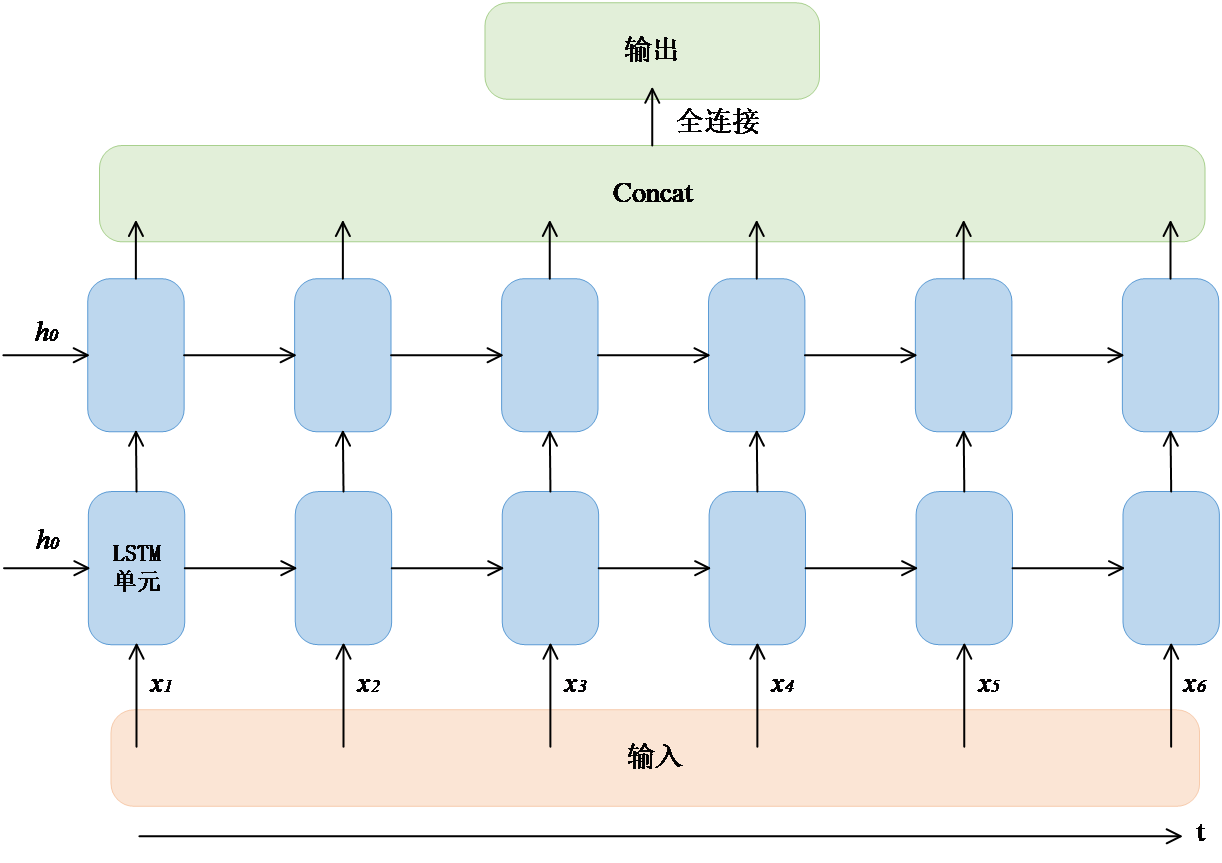
\includegraphics[scale=0.6]{figures/lstm.png}
    \caption{LSTM网络结构图}
    \label{fig:lstm}
\end{figure}

训练集按照样本维度进行了归一化(零均值化和方差归一化),并按照训练集上的参数对验证集和
测试集进行同样的归一化操作,以使数据尺度相同。

\subsection{集成方法}
三个臭皮匠顶个诸葛亮。在集成方法中,我们训练多个弱学习器模型以解决相同的问题,并将它们结合起来从而获得更好的结果。当弱学习期被正确组合时,可以得到更精确更鲁棒的模型。在bagging和boosting等方法中,我们使用多个同一种基学习器,加入随机因子,用不同的方法训练;也可以使用不同种类的基学习器。
\subsubsection{平均方法average}
投票分类器是将不同的基学习器组合,并使用多数表决或平均预测概率来预测类标签。这样的分类器可用于一组性能良好的模型,以平衡其各自的弱点。
本文采用单独模型中的LR、SVM、KNN、RF、MLP生成组合模型,分别采用多数表决(hard)和平均预测概率(soft)两种方法实现。
用sklearn包中votingclassifier实现。

\subsubsection{Bagging}
用Bagging方法训练多个单独的分类器,并将分类器进行组合,以实现一个更强性能的大分类器。

\section{实验设计及结果}

\subsection{训练集、验证、测试集的划分}
由于天气特性与地理位置之间具有强的相关性,所以处于不同地理位置上的气象站的天气指标
具有不同的分布特点,为了能够对各个气象站所在位置的降雨量进行更加精准的建模和预测,
对每个气象站的降雨量预测任务单独建模。将每个气象站的天气数据按照时间顺序以7:2:1的比例
划分为训练集、验证集和测试集。

为了避免训练集和验证、测试集中的数据出现交叉,影响模型性能的判断,先将清洗过后的数据拆分为
不同集合,然后在每个集合中分别进行窗口滑动,从第一个有记录的时刻开始,窗口滑动的步伐为1,当前时刻到
之后的连续第6个时刻的数据样本作为一个样本,第7时刻的降雨量类别作为该样本的目标值。


\subsection{评价指标的定义}
本次任务是一种多分类任务,所以选择以下四种评价指标对模型预测能力进行判别:
\begin{enumerate}
    \item 准确率(accuracy):即分类正确的样本数站总样本数的比例,这是最为常用的分类问题评价标准
    ,但是对于本问题中类别不平衡的数据集该评价指标不能有效说明分类器的预测性能,因为数据中降雨量类别
    为0的数据占90\%左右,即使模型给出全0的结果也可以得到比较高的accuracy。
    \item 精确率(precision):二分类问题中,被关注的类的精确率计算方式为$p=\frac{TP}{TP+FP}$,本问题
    为一个多分类问题,计算各类的加权平均精确率作为多类别分类器在测试集上的最终精确率。
    \item 召回率(recall):与精确率的计算方式类似,计算各类的召回率$r=\frac{TP}{TP+FN}$,将各类的
    加权平均召回率作为模型在测试集上的最终召回率。
    \item f1-score:精确率和召回率是一对相互矛盾的量,有着相反的变化趋势,所以为了能够更好的评价
    分类器的性能,使用f1-score$= \frac{2\times p\times r}{p+r}$评价分类器的综合性能,多分类器的f1-score
    为各类该指标的加权平均。
\end{enumerate}

\subsection{单独模型的最好结果对比}
XGBoost和LSTM均为在清洗过后的数据上进行实验,并且对每个气象站进行建模时,
去掉了整个数据中为常量,或者冗余的特征变量,在章节\ref{feature_subset}的基础上保留了对应的max和min特征,共21个特征变量。

LSTM网络模型在迭代20次之后,损失函数就呈现非常缓慢的下降,继续增加迭代次数对最终模型的
性能影响不大,所以共迭代30次。

从表\ref{tab:single_model}所示,共九种模型的四个指标。每一个单元格中从左到右分别为371-375五个气象站的结果,可以看到在同一个气象站数据下,不同模型的四个指标都有类似的数值,即不同气象站的指标具有不同的均值和方差,说明分类结果与数据集本身分布相关。综合来看模型中树模型GBDT和\\XGBoost的性能相对最优。整体来看,各个模型的性能指标都类似,只有小幅的偏差,可能说明分类器的性能均已达到比较优的情况。另外,在accuracy,precision,recall,fscore里,precision和fscore数值上相对稍低,recall相对稍高。

\begin{table}[htb]
    \centering
    \begin{minipage}[t]{\linewidth}
    \centering
    \caption{单独模型的最好结果对比}
    \label{tab:single_model}
      \begin{tabular}{ccccc}
        \toprule[1pt]
        模型 & accuracy & precision & recall & f1-score \\
        \midrule[0.5pt]
        LR & .93|.93 |.89|.96|.95 & .90|.90|.83|.93|.93& .93|.93|.89|.96|.95& .91|.91|.84|.94|.93 \\
        SVM & .93|.93|.89|.96|.95& .91|.90|.84|.93|.92& .93|.93|.89|.96|.95 & .91|.91|.85|.94|.92 \\
        KNN & .93|.92|.88|.96|.95 & .90| .89|.83|.93|.91& .93|.93|.88|.96|.94& .91|.90|.85|.94|.92 \\
        DT & .93|.93|.90|.96|.95 &.91|.92|.87|.95|.93& .93|.93|.90|.96|.95& .92|.92|.88|.95|.94 \\
        RF & .93|.93|.90|.96|.94 & .91|.91|.87|.94|.93 & .93|.93|.90|.95|.94 & .92|.92|.88|.95 |.94\\
        GBDT & .94|.93|.90|.96|.95 &.92|.92|.88|.95|.94& .94|.93|.90 |.96|.95 & .93|.92|.89|.95|.94 \\
        MLP & .94|.93|.90|.96|.95 &.92|.91|.87|.95|.94& .94|.93|.90|.96|.95& .93|.92|.88|.95|.94 \\
        XGBoost & .93 |.93|.90|.95|.95 & .92|.92|.87|.93|.94 & .93|.93|.90|.95|.95 & .92|.92|.88|.94|.94 \\
        LSTM & .93|.93|.88|.95|.95 & .86|.86|.78|.89|.89  & .93|.93|.88|.95|.95 & .90|.90|.83|.92|.92 \\
        \bottomrule[1pt]
      \end{tabular}
    \end{minipage}
  \end{table}

\subsection{集成模型的最好结果对比}
用Bagging方法对XGBoost模型进行集成,每一次从训练集中有放回的随机抽取和训练集一样大小的子训练集,用
该子训练集训练一个相对简单的XGBoost分类器,并重复以上过程$n$次,最终得到$n$个相对较弱的XGBoost分类器,
并基于投票的思想将$n$个弱分类器组成一个大的分类器,用验证集对该分类器进行验证,选择最好的分类器。
用投票法对不同基学习器,包括LR、SVM、KNN、RF、MLP进行集成,具体结果见表\ref{tab:ensemble_model}

\begin{table}[htb]
  \centering
  \begin{minipage}[t]{\linewidth}
  \centering
  \caption{集成模型的最好结果对比}
  \label{tab:ensemble_model}
    \begin{tabular}{ccccc}
      \toprule[1pt]
      模型 & accuracy & precision & recall & f1-score \\
      \midrule[0.5pt]
      Bagging-XGBoost & .94|.93|.90|.95|.95 & .92|.92|.87|.93|.94 & .94|.93|.90|.95|.95 & .92|.92|.88|.94|.94 \\
      hard-voting & .93|.94|.89|.95|.95 & .90|.91|.85|.92|.92 & .93|.94|.89|.95|.95 & .91|.92|.86|.93|.93 \\
      \bottomrule[1pt]
    \end{tabular}
  \end{minipage}
\end{table}

可以看到用多个由随机子训练集训练得到的XGBoost组合分类器在该问题上的性能和单独的最优XGBoost分类器并无显著差别。不同基学习器组成的投票分类器与单独模型同样并无显著差别,甚至还略有下降,可能是不稳定模型反而降低了稳定模型的性能,也可能是因为单个模型已经有很好的性能了。
同样的bagging方法,在随机子训练集上训练得到了多个LSTM分类器,并组成一个大的分类器,该分类器在测试集上的分类性能与单独的最优LSTM相比几乎没有提高,
仍然出现了非常严重的类别不平衡带来的问题,组合分类器对无雨类别的样本能够给出高精度的预测结果,但是对于其他类别的样本几乎没有预测能力,精确率和召回率都为0,故此处不再给出单独用多个LSTM组合而成的大分类器具体表现结果。


\subsection{每种模型在不同超参数下的表现}
\subsubsection{XGBoost}
最初用XGBoost模型对每一个气象站的数据分别调参,希望对每一个气象站分别得到一个最优超参数。
在实验过程中,发现XGBoost模型性能在该问题上对超参数的选择不敏感,每一个气象站的训练学习率从0.01到0.2调整,
决策树最大深度从5到10变化,决策树个数从10到500变化,分别用单独的气象站数据训练得到的模型在验证集上的
实验结果几乎没有差别,所以可以在流程上进行简化,对所有的气象站数据分别用同一组超参数进行训练,并为了节省模型的训练时间
和测试时间,将模型超参数的设置在保证模型性能的基础上使最终模型尽可能的小。

\subsubsection{LSTM}
LSTM模型的超参数有LSTM层数、隐层变量数以及训练过程的学习率上,通过多次实验进行选择,发现LSTM层数的增多对最终模型的拟合能力
的提高没有明显的贡献,所以设置LSTM的层数为2,全连接层的增加也无法提高模型的拟合能力,所以在最后一层的
LSTM输出以上设置一个全连接层,LSTM单元的隐变量个数均为10。
最初选择用带有动量项的随机梯度下降方法训练,无论怎样设置学习率和动量因子,模型都非常缓慢的收敛,
最终选择了可以在训练过程中通过计算梯度的一阶矩估计和二阶矩估计而不断自适应更新学习率的Adam算法。
调整初始的学习率发现,该训练过程对初始学习率的设置并不敏感,使学习率从0.01到0.2变化,
模型训练速度基本相同,都能在30次迭代后基本达到收敛状态。

\subsubsection{经典模型}
LR、SVM、KNN、DT、RF等均为机器学习经典模型,且在上课和课后作业中讨论过不同超参数的影响,不再赘述。此节讨论class\_weight这一参数对模型的影响。

由章节\ref{sec:data}可知降水量数据具有稀疏性,导致分类后样本极度不均衡,由此训练出的分类器可能有较高的准确性但是性能较差。为了解决这一问题,可以采用以下几种措施:

\begin{itemize}
	\item 扩大数据集,对稀有样本重采样,对多数样本进行欠采样;
	\item 采用更合理的评价指标,比如本文中采用的precision、recall和f1-score;
	\item 尝试不同的分类算法,比如决策树模型等常在类别不均衡的问题上有较好的表现;
	\item 对问题重新定义,可将小类样本作为异常点,因此该问题即转化为异常点检测(anomaly detection)与变化趋势检测问题(change detection);
	\item 采用代价敏感学习方法,给少数类样本分配较高的误分类代价,而给多数类样本分配较小的误分类代价,通过这种方式在训练中人为提高了少数类别样本的重要性,以此减轻分类器对多数类的偏好。
	\item 采用集成方法。

\end{itemize}

本文对LR,SVM,DT三种算法进行样本均衡,设置class\_weight参数为‘balanced’,根据样本数量确定权重,以372气象站为例,得到结果如下表\ref{tab:class}所示。
可以看到LR对样本均衡问题不敏感,而SVM和DT则有较大变化。SVM增加了样本权重后,accuracy大幅降低,precision稍有上升,recall和fscore均下降。DT同样accuracy大幅降低,precision,recall和fscore均下降。这是由模型特点决定的,LR不会受到小噪声的影响;SVM对于不同代价函数敏感,可能会导致不同的边界和支持向量;单棵DT由于样本不均衡会产生一定的偏向,这一问题能够在森林中解决。
另外,对于数据集的进一步清洗,包括删除缺失属性的数据条等操作,能够提高balanced后的模型性能,这可能是因为清洗的绝大部分是0类,一定程度上改善了样本不均衡的问题。

\begin{table}[htb]
  \centering
  \begin{minipage}[t]{\linewidth}
  \centering
  \caption{class\_weight超参数结果对比}
  \label{tab:class}
    \begin{tabular}{ccccc}
      \toprule[1pt]
      模型 & accuracy & precision & recall & f1-score \\
      \midrule[0.5pt]
      LR & .93 & .90 & .93 & .91\\
      LR(balanced) &  .91 & .92 &.91 &.92 \\
      SVM &.93 &.9 &.93 & .91   \\
      SVM(balanced) & .79 & .92& .79& .84 \\
      DT & .93 & .92 & .93 & .92\\
      DT(balanced) & .83 &.91 &.83 &.87 \\
      \bottomrule[1pt]
    \end{tabular}
  \end{minipage}
\end{table}

\subsection{其他实验设计及结果}
\subsubsection{LSTM的easyensemble方法}
在实验中发现LSTM模型对这种类别不平衡问题表现的不好,特别是对于数据较少的类别,所以希望能够通过一些减少类别不平衡
问题的操作,提高LSTM模型对该问题的拟合能力和预测能力。EasyEnsemble算法是一种用于处理类别不平衡问题
的欠采样算法,在本问题上该算法的实现步骤如下:
\begin{enumerate}[(1)]
  \item 从无雨的类别数据中又放回的随机采样$n$次,每次选取与其他类别数据数目相近的
  样本个数,最后得到$n$个用子样本集合$\{S_1, S_2, \dots, S_n\}$。
  \item 分别将以上$n$个子样本集合与其他类别的数据样本合并为$n$个子训练集,并
  用每个子训练集训练出一个LSTM模型,如此可得到$n$个模型。
  \item 将这$n$个模型组合成一个集成学习系统,最终用这$n$个模型的结果进行投票。
\end{enumerate}

在实验中,将每次对无雨的类别数据采样数据为其他类别数据总和的0.4倍,一共生成100个子训练集,从而
训练得到100个子分类器。不过得到的训练器整体性能与单独的LSTM模型相比并没有提升,反而下降。
以在气象站373上用EasyEnsemble方法训练得到的多LSTM模型组成的大分类器为例,该分类器在测试集上的实验结果
如表\ref{tab:easyensemble}中所示。


\begin{table}[htb]
  \centering
  \begin{minipage}[t]{\linewidth}
  \centering
  \caption{EasyEnsemble方法在气象站373测试集上的实验结果}
  \label{tab:easyensemble}
    \begin{tabular}{ccccc}
      \toprule[1pt]
      类别 & precision & recall & f1-score & 样本量\\
      \midrule[0.5pt]
      无雨(0) & 0.97 & 0.50 & 0.66 & 7046\\
      小雨(1) & 0.12 & 0.89 & 0.22 & 595 \\
      中雨(2) & 0.00 & 0.00 & 0.00 & 228 \\
      大雨到暴雨(3) & 0.00 & 0.00 & 0.00 & 95\\
      加权平均 & 0.87 & 0.51 & 0.60 & 7964\\
      \bottomrule[1pt]
    \end{tabular}
  \end{minipage}
\end{table}

该分类器在测试集上的预测准确率为0.51,相比于表\ref{tab:single_model}中单独LSTM模型的预测性能,
该分类器的性能变弱了。precision,recall和f1-score的加权平均值都比单独LSTM模型的测试结果小,
但是分开看各个类别的预测结果,其中表\ref{tab:easyensemble}中显示该分类器对小雨类别的数据预测
recall为0.89,这个是明显强于单独LSTM模型的,前面已经介绍过,用所有训练数据得到的单独LSTM模型除了对
无雨类别数据能给出很高的预测结果,其他类别的数据预测能力几乎为0,即其他类别的评价值均为0。而用EasyEnsemble
对无雨类别数据欠采样得到的大分类器能够对小雨类别的数据有一定的预测能力,这是该方法于单独LSTM方法提高的点,
这说明用EasyEnsemble方法得到的一系列子分类器组成的大分类器在一定程度上能够缓解类别不平衡问题,不过只是在
一定程度上。如表\ref{tab:easyensemble}中中雨和大雨到暴雨类别的数据分类器预测的评价指标仍均为0,分析原因可能
是因为小雨类别的数据要显著高于中雨和大雨到暴雨这两类,在对无雨类别数据欠采样后,子训练集中小雨和无雨两类数据
占比较高,而另外两种就占比很少,所以最终得到的分类器对后面两类不能给出正确的预测结果,所以这样看来,
采用EasyEnsemble算法只在一定程度上解决了部分类别不平衡的问题,由于四类数据之间的样本量差距都比较大,所以
无法用这种对多类数据欠采样的方法来从根本上解决这个问题,而且由于欠采样后子训练集中的样本量较少,难以用来
训练得到较为高性能的LSTM模型,进而得到的大分类器性能也较差,故该实验没有在ensemble部分进行报告。

\subsubsection{不同数据集上模型的迁移能力}
尝试用在气象站371上训练的分类器在其他四个气象站372-375测试集上测试,具体表现如下表\ref{tab:transfer}所示。模型选择最优的GBDT。由此可见五个气象站数据之间有很强的相似性,在气象站371上训练得到的分类器,在其他几个气象站上表现也很不错。

\begin{table}[htb]
  \centering
  \begin{minipage}[t]{0.9\linewidth}
  \centering
  \caption{不同数据集上模型的迁移能力}
  \label{tab:transfer}
    \begin{tabular}{ccccc}
      \toprule[1pt]
      模型 & accuracy & precision & recall & f1-score \\
      \midrule[0.5pt]
      station1 & .94 & .92 & .94 & .93\\
      station2 &  .93 & .91 & .93 &.92 \\
      station3 &.90 & .86 & .90 & .87  \\
      station4 & .95 & .94& .95& .94 \\
      station5 & .91 & .93 & .91 & .92\\
      \bottomrule[1pt]
    \end{tabular}
  \end{minipage}
\end{table}



\section{结果分析与讨论}
\subsection{数据和模型中每一部分的贡献}
在本项目中,我们分别对每一个气象站的降雨与其他气象特征单独建模,
用前六时刻的气象特征预测下一时刻的降雨可能性与降雨量大小。数据特征的选取
及各特征与目标变量之间的相关性分析可见下一节中关于特征的具体分析。

下面分别讨论各个模型在解决降雨量预测问题上的作用。
\begin{enumerate}
  \item XGBoost模型是一种基于Adaboost思想的决策树森林,森林中的树按照串行关系依次用
  训练集训练得到,每个树的优化目标都与之前已生成的决策树有关。最后得到的XGBoost
  模型包含多个子分类器,在对输入进行预测时,每个子分类器都给出各自的预测结果,最后
  所有子分类器进行投票,最终给出XGBoost模型的分类结果。
  \item LSTM模型是一种循环神经网络模型,与其他的算法不同,使用该模型进行降雨量
  预测无需将$T\times P$格式的二维矩阵展开为一维向量,按照时间顺序将$T$个时刻
  的特征向量依次输入到LSTM网络中。用于降雨量预测的LSTM模型由两部分组成,输入的特征向量
  先经过两层LSTM网络进行特征提取,第二层LSTM网络的输入为一个长度固定的向量,该向量再输入一个
  全连接网络中,用于给出分类结果。在整个LSTM模型中,两层LSTM网络作为一个特征提取的过程,
  并将特征用一个固定长度的向量来表示,后面的全连接网络作为结果预测部分,用提取到的特征对最后
  分类结果进行预测。
\end{enumerate}


\subsection{特征的重要性分析}
\label{sec:all features}
利用随机森林分类结果,可以得到特征重要性排序,前十个特征由下表\ref
{tab:rf}所示,其中特征前的数字表示前$6-n$小时的值。
\begin{table}[htb]
  \centering
  \begin{minipage}[t]{0.9\linewidth}
  \centering
  \caption{特征重要性分析}
  \label{tab:rf}
    \begin{tabular}{ccc}
      \toprule[1pt]
       & 特征 & 重要性  \\
      \midrule[0.5pt]
      1 & 5prcp & 0.217  \\
      2 & 4prcp & 0.156 \\
      3 & 3prcp & 0.143  \\
      4 & 2prcp & 0.097\\
	  5 & 5hmdy & 0.016  \\
	  6 & 5gbrd & 0.016  \\
      7 & 4hmdy & 0.016 \\
      8 & 5temp & 0.015\\
	  9 & 5wdct & 0.014  \\
      10 & 4gbrd & 0.012 \\
      \bottomrule[1pt]
    \end{tabular}
  \end{minipage}
\end{table}


上述结果均由用章节\ref{feature_subset}的特征子集得到,考虑把所有数值特征不经过特征选择,直接输入模型中,可以观察到结果基本相似,甚至略有提升。这可能是因为max和min值增加了信息,使预测更准确。

另外,不清洗缺失某些数据值的数据条,也会得到略有提升的模型性能。可能是因为缺失的特征对于分类的重要性不高,保留使得数据集样本规模更大,所以会有更好的性能。


\subsection{错误分析}

如前面所介绍过的,由于实验中所采用的地区降雨都为小概率时间,所以大部分时间都为无雨状态。即使下雨,
大部分情况为小雨,中雨出现次数更少,而大雨的概率就极低。使得该问题中不同类别的数据样本量差别极大,
属于严重类别不平衡的情况。无雨的类别占比能达到90\%以上,所以用该数据训练得到的预测模型,对于无雨的
情况能够给精确度和召回率都非常高的预测结果,而对于其他三种类型的数据预测能力就会弱很多。
为了具体说明这种情况的普遍性,表\ref{tab:xgb-375}示出了气象站375上的最优XGBoost模型在其测试集上的
实验结果。
在该数据集上,无雨的样本占据94.6\%,其他三类数据共占据5.4\%。
无雨类别的precision和recall值分别为0.96,0.99,f1-score为0.98,都非常高,
说明该该模型对无雨类别的数据有很高的拟合能力,这与训练集中绝大部分样本也为无雨类别有关。
而测试集中小雨、中雨和大雨类别的f1-score值都在0.5以下,这说明该模型对于这三类样本的拟合能力比较弱,
特别是对雨样本量不足2\%的中雨和大雨两类,预测能力非常弱。

类别不均衡带来的分类器在不同类别上表现具有巨大差异的问题在LSTM模型上更为明显,除了在气象站373上的模型,
其他气象站的LSTM模型在测试集上中无雨类别上的f1-score均可达到0.95及以上(气象站373为0.94),
而在其他类别上的precision和recall几乎都为零,即LSTM模型完全无法对这种在训练集中占比极低的样本进行拟合。


\begin{table}[htb]
  \centering
  \begin{minipage}[t]{\linewidth}
  \centering
  \caption{最优XGBoost模型在气象站375上的测试结果}
  \label{tab:xgb-375}
    \begin{tabular}{ccccc}
      \toprule[1pt]
      类别 & precision & recall & f1-score & 样本量\\
      \midrule[0.5pt]
      无雨(0) & 0.96 & 0.99 & 0.98 & 7992\\
      小雨(1) & 0.46 & 0.26 & 0.34 & 330 \\
      中雨(2) & 0.27 & 0.07 & 0.12 & 95 \\
      大雨到暴雨(3) & 0.75 & 0.09 & 0.15 & 35\\
      \bottomrule[1pt]
    \end{tabular}
  \end{minipage}
\end{table}

\section{代码说明}
\subsection{参考代码}
数据清洗部分主要参考了kaggle上的两个notebook:\cite{bit7}和\cite{big8}。


\subsection{代码使用说明}
代码具体使用方式请见文件README.md。

\section{小组成员贡献}
\textbf{张芙作}
  \begin{enumerate}
    \item 文献调研,调研降雨量预测问题的主流解决方法;
    \item 调研用机器学习模型处理时空序列问题的方法;
    \item 用XGBoost模型实现降雨量预测及实验验证;
    \item 实现LSTM模型预测降雨量及实验验证;
    \item 用Bagging方法对单独的XGBoost模型和LSTM模型进行集成及实验验证;
    \item 调研类别不均衡结局方案,并用EasyEnsemble方法集成LSTM
    模型并实验验证;
    \item 合作报告撰写。
  \end{enumerate}

\textbf{孟诗涵}

\section{结论}
本文基于巴西降水量数据集用线性模型、树模型和神经网络模型进行了降水量预测分类实验,设计了多种实验并对实验结果进行了分析,得到以下结论:
\begin{itemize}
\item 在同一个气象站数据下,不同模型的四个评价指标都有类似的数值,即不同气象站的指标具有不同的均值和方差,说明分类结果与数据集本身分布相关。
\item 九种模型的性能类似,相对而言GBDT和XGBoost性能最优,LSTM性能最差。Ensemble组合分类器与单一模型相比性能没有明显提升,甚至略有下降。
\item 数据集有明显的样本不均衡问题,尝试并讨论了LR、SVM、DT中class\_weight这一超参数的作用,以及LSTM中的EasyEnsemble方法,均不能很好的解决不均衡的问题。说明成功的机器学习分类器基于良好的结构化的数据集,要重视数据集的清洗处理等工作。
\item 分类结果对选取的特征不敏感,13维的特征子集和21维的特征子集结果相似。
\end{itemize}

\begin{thebibliography}{20}
  \bibitem{bit1} 周泽世. 基于BP神经网络的降雨量预测研究[D].湖南农业大学, 2015.
	\bibitem{bit2} Yuxuan Liang, Songyu Ke, Junbo Zhang, Xiuwen Yi, Yu Zheng, GeoMAN: Multi-level Attention Networks
  for Geo-sensory Time Series Prediction. In International Joint Conference on Artificial Intelligence(IJCAI), 2018.
  \bibitem{bit3} Yu Zheng, Xiuwen Yi, Ming Li, Ruiyuan Li, Zhangqing Shan, Eric Chang, and Tianrui Li. Forecasting finegrained air quality based on big data. In Proceedings of the 21th ACM SIGKDD International Conference
  on Knowledge Discovery and Data Mining, pages 2267–2276. ACM, 2015.
  \bibitem{bit4} Ramana R V, Krishna B, Kumar S R, et al. Monthly rainfall prediction using wavelet neural network
  analysis[J]. Water resources management, 2013, 27(10): 3697-3711.
  \bibitem{bit5} Junbo Zhang, Yu Zheng, Dekang Qi, Ruiyuan Li, and Xiuwen Yi. Dnn-based prediction model
  for spatio-temporal data. ACM SIGSPATIAL 2016, October 2016.
  \bibitem{bit6} Hourly weather surface, Kaggle. \url{https://www.kaggle.com/PROPPG-PPG/hourly-weather-surface-brazil-southeast-region}.
  \bibitem{bit7} https://www.kaggle.com/dedecu/cross-correlation-time-lag-with-pandas
  \bibitem{bit8} https://www.kaggle.com/sanjayroberts1/exploratory-data-analysis-and-clean-up
\end{thebibliography}


\end{document}
